% This is text associated with the open textbook "Open Electromagnetics"
% See immediately below for author, date
% This work is licensed under the Creative Commons Attribution-ShareAlike 4.0 International License. (CC BY-SA 4.0) 
% To view a copy of the license, visit http://creativecommons.org/licenses/by-sa/4.0/

%ORB TITLE Potential Field Within a Parallel Plate Capacitor
%ORB AUTHOR 0        # S.W. Ellingson, Virginia Tech (ellingson@vt.edu)
%ORB DATE 20180806   # yyyymmdd
%ORB ABSTRACT The Electric Potential Field Within a Parallel Plate Capacitor Using Laplace's Equation

\label{m0068_V_Within_Parallel_Plate_Cap_Using_Laplaces_Equation} % <-- Must match name of this file and module directory name.  Don't mess with this!
\index{capacitor!parallel plate|(}

This section presents a simple example that demonstrates the use of Laplace's Equation 
\index{Laplace's equation}
(Section~\ref{m0067_Poissons_and_Laplaces_Equations}) to determine the potential field in a source free region.
The example, shown in Figure~\ref{m0068_fPPC}, pertains to an important structure in electromagnetic theory -- the parallel plate capacitor.
Here we are concerned only with the potential field $V({\bf r})$ between the plates of the capacitor; you do not need to be familiar with capacitance or capacitors to follow this section (although you're welcome to look ahead to Section~\ref{m0112_Capacitance} for a preview, if desired). 
What \emph{is} recommended before beginning is a review of the battery-charged capacitor experiment discussed in Section~\ref{m0002_Electric_Field_Intensity}. In this section you'll see a rigorous derivation of what we figured out in an informal way in that section. 

The parallel-plate capacitor in Figure~\ref{m0068_fPPC} consists of two perfectly-conducting circular disks separated by a distance $d$ by a spacer material having permittivity $\epsilon$. 
There is no charge present in the spacer material, so Laplace's Equation applies.
That equation is (Section~\ref{m0067_Poissons_and_Laplaces_Equations}):
\begin{equation}
\nabla^2 V = 0 ~~\mbox{(source-free region)}
\label{m0068_eLaplace}
\end{equation}
%
Let $V_C$ be the potential difference between the plates, which would also be the potential difference across the terminals of the capacitor.
The radius $a$ of the plates is larger than $d$ by enough that we may neglect what is going on at at the edges of the plates -- more on this will be said as we work the problem.
Under this assumption, what is the electric potential field $V({\bf r})$ between the plates?   
%
\begin{figure}
\begin{center}
\pdftooltip{{  % note double braces
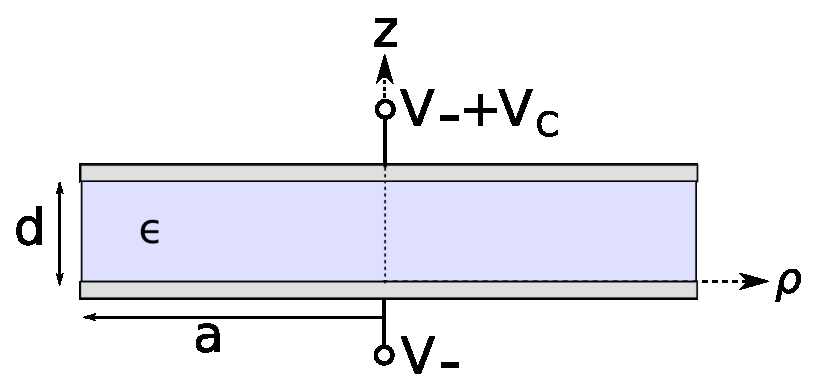
\includegraphics[width=2.5in]{modules/m0068_fPPC.eps}
}}{A parallel plate capacitor, oriented horizontally, with a node above and below the capacitor on the vertical z-axis. The top node is labeled V sub minus plus V sub C. The bottom node is labeled V sub minus. The thin plates on top and bottom are represented by silver lines, and the spacer material between colored blue and labeled epsilon. The distance between the plates is labeled d. From the origin of the z-axis, an arrow extends to the left side of the capacitor, labeled a.  From the origin z-axis pointing to the right, a dashed arrow is labeled rho.}
\end{center} 
\caption{
\label{m0068_fPPC} 
A parallel plate capacitor, as a demonstration of the use of Laplace's Equation.
}
\end{figure}

This problem has cylindrical symmetry, so it makes sense to continue to use cylindrical coordinates with the $z$ axis being perpendicular to the plates.
Equation~\ref{m0068_eLaplace} in cylindrical coordinates is:
%
\begin{equation}
\left[ \frac{1}{\rho} \frac{\partial}{\partial \rho} \left( \rho \frac{\partial}{\partial \rho} \right) 
+ \frac{1}{\rho^2} \frac{\partial^2}{\partial \phi^2}
+ \frac{\partial^2}{\partial z^2} \right] V
= 0 
\end{equation}
%
or perhaps a little more clearly written as follows:
%
\begin{equation}
\frac{1}{\rho} \frac{\partial }{\partial \rho} \left( \rho \frac{\partial V}{\partial \rho} \right) 
+ \frac{1}{\rho^2} \frac{\partial^2 V}{\partial \phi^2}
+ \frac{\partial^2 V}{\partial z^2} 
= 0 
\end{equation}
%
Since the problem has radial symmetry, $\partial V/\partial \phi = 0$.
Since $d \ll a$, we expect the fields to be approximately constant with $\rho$ until we get close to the edge of the plates.
Therefore, we assume $\partial V/\partial \rho$ is negligible and can be taken to be zero. 
Thus, we are left with 
%
\begin{equation}
\frac{\partial^2 V}{\partial z^2} \approx 0 ~~ \mbox{for $\rho \ll a$} 
\label{m0068_eDE}
\end{equation}

The general solution to Equation~\ref{m0068_eDE} is obtained simply by integrating both sides twice, yielding
%
\begin{equation}
V(z) = c_1 z + c_2
\label{m0068_eVAC} 
\end{equation}
%
where $c_1$ and $c_2$ are constants that must be consistent with the boundary conditions. 
Thus, we must develop appropriate boundary conditions.
Let the node voltage at the negative ($z=0$) terminal be $V_{-}$.  
Then the voltage at the positive ($z=+d$) terminal is $V_{-}+V_C$.  
Therefore:
%
\begin{flalign}
V(z=0)  &= V_{-} \\
V(z=+d) &= V_{-}+V_C 
\end{flalign}
%
These are the relevant boundary conditions.  
Substituting $V(z=0) = V_{-}$ into Equation~\ref{m0068_eVAC} yields $c_2 = V_{-}$.
Substituting $V(z=+d) = V_{-}+V_C$ into Equation~\ref{m0068_eVAC} yields $c_1 = V_C/d$.  
Thus, the answer to the problem is
%
\begin{equation}
V(z) \approx \frac{V_C}{d} z + V_{-}  ~~ \mbox{for $\rho \ll a$} 
\label{eEP-PEPP1}
\end{equation}
%
Note that the above result is dimensionally correct and confirms that the potential deep inside a ``thin'' parallel plate capacitor changes linearly with distance between the plates.

Further, you should find that application of the equation ${\bf E} = - \nabla V$ (Section~\ref{m0063_Electric_Field_as_the_Gradient_of_Potential}) to the solution above yields the expected result for the electric field intensity: ${\bf E} \approx -\hat{\bf z}V_C/d$.  
This is precisely the result that we arrived at (without the aid of Laplace's Equation) in Section~\ref{m0002_Electric_Field_Intensity}.   

A reasonable question to ask at this point would be, what about the potential field close to the edge of the plates, or, for that matter, beyond the plates?  
The field in this region is referred to as a \emph{fringing field}. 
\index{fringing (field)}
For the fringing field, $\partial V/ \partial \rho$ is no longer negligible and must be taken into account.  In addition, it is necessary to modify the boundary conditions to account for the outside surfaces of the plates (that is, the sides of the plates that face away from the dielectric) and to account for the effect of the boundary between the spacer material and free space. 
These issues make the problem much more difficult.
When an accurate calculation of a fringing field is necessary, it is common to resort to a numerical solution of Laplace's Equation.
Fortunately, accurate calculation of fringing fields is usually not required in practical engineering applications.

\index{capacitor!parallel plate|)}
